%\documentclass[preprint]{sigproc}
\documentclass{acm_proc_article-sp}

% The following \documentclass options may be useful:
%
% 10pt          To set in 10-point type instead of 9-point.
% 11pt          To set in 11-point type instead of 9-point.
% authoryear    To obtain author/year citation style instead of numeric.

\setlength{\textfloatsep}{5pt}

\usepackage{flushend}
\usepackage{graphicx}
\usepackage{verbatim}
\usepackage{url}
\usepackage{alltt}
\renewcommand{\ttdefault}{txtt}

\usepackage{amsmath}
\usepackage{dsfont}
\usepackage{mathtools}
\everymath{\displaystyle}
\usepackage{xspace}

\newcommand{\CEU}{\textsc{C\'{e}u}\xspace}
\newcommand{\code}[1] {{\small{\texttt{#1}}}}
\newcommand{\DOFIN}{\code{do-finally}\xspace}
\newcommand{\FIN}{\code{finally}\xspace}

\newcommand{\ST}{\1\xrightarrow[~n~]{}\1}
\newcommand{\BT}{\xRightarrow[(i,E)]{}}
\newcommand{\LL}{\langle}
\newcommand{\RR}{\rangle}
\newcommand{\DS}{\displaystyle}
\newcommand{\rr}[1] {{\textbf{\scriptsize{#1}}}}


\newcommand{\1}{\;}
\newcommand{\2}{\;\;}
\newcommand{\3}{\;\;\;}
\newcommand{\5}{\;\;\;\;\;}
\newcommand{\ten}{\5\5}
\newcommand{\twenty}{\ten\ten}

\newenvironment{itemize*}%
  {\begin{itemize}%
    \setlength{\itemsep}{0pt}%
    \setlength{\parskip}{0pt}}%
  {\end{itemize}}

\usepackage{enumitem}
\setlist{nolistsep}

\usepackage{color}
\definecolor{light}{gray}{0.87}
\definecolor{dark}{gray}{0.30}
%\definecolor{light}{rgb}{.90,.90,.90}
\definecolor{darkgreen}{rgb}{0,.50,0}
\definecolor{darkblue}{rgb}{0,0,.50}
\definecolor{darkred}{rgb}{.50,0,0}
\definecolor{darkpur}{rgb}{.50,0,.50}

\usepackage{listings}
%\usepackage{textcomp}
\lstset{
%columns=fullflexible,
%basicstyle=\ttfamily,
escapeinside={||},
mathescape=true,
    language=C, % choose the language of the code
    basicstyle=\fontfamily{pcr}\selectfont\scriptsize\color{black},
    keywordstyle=\color{black}\bfseries, % style for keywords
    numbers=none, % where to put the line-numbers
    numberstyle=\tiny, % the size of the fonts that are used for the line-numbers
    backgroundcolor=\color{light},
    showspaces=false, % show spaces adding particular underscores
    showstringspaces=false, % underline spaces within strings
    showtabs=false, % show tabs within strings adding particular underscores
    %frame=single, % adds a frame around the code
    tabsize=2, % sets default tabsize to 2 spaces
    %rulesepcolor=\color{gray}
    captionpos=t, % sets the caption-position to bottom
    breaklines=false, % sets automatic line breaking
    %breakatwhitespace=false,
    numbersep=2em,
    emph={par,or,hor,do,end,loop,await,emit,input,event,call,with,command,%
          var,and,then,else,C,return,pure,deterministic,nohold,finalize,%
          each, abort, when, signal, PROC, CHAN, SIGNAL, PAR},
    emphstyle={\bfseries},
    commentstyle=\color{dark}\scriptsize,
    %xleftmargin=20pt,
    %xrightmargin=20pt,
    framesep=20pt,
    %upquote=true,
    %aboveskip={1.5\baselineskip},
}

\begin{document}

\title {
    %Imperative and Synchronous Abstractions for Reactive Applications
    Structured Reactive Programming
}
%\subtitle{Accepted paper in REM'13 (preprint version)}

- rely on the synchronous execution model
- compositions
- than abstracting over it
- finalization, safety
- ortoghonal preemption
- simple reasoning

- OS/drivers are stateful

\numberofauthors{1}
\author{
    \alignauthor
    Francisco Sant'Anna \hspace{1cm} Noemi Rodriguez \hspace{1cm} Roberto Ierusalimschy   \\
    \affaddr{Departamento de Inform\'atica --- PUC-Rio, Brasil} \\
    \email{\{fsantanna,noemi,roberto\}@inf.puc-rio.br}
}

\maketitle

\begin{abstract}
Reactive applications interact in real time and continuously with external 
stimuli from the surrounding environment.
They represent a wide range of software areas and platforms: from games in 
powerful desktops, \emph{"apps"} in capable smart phones, to the emerging 
internet of things in constrained embedded systems.

Research on special-purpose reactive languages dates back to the early 80's 
with the co-development of two complementary styles~\cite{rp.twelve}:
%
The imperative style of Esterel~\cite{TODO} organizes programs with control 
flow primitives, such as sequences, repetitions, and also parallelism.
%
The dataflow style of Lustre~\cite{TODO} represents programs as graphs of 
values, in which a change to a node updates its dependencies automatically.

In recent years, Functional Reactive Programming~\cite{TODO} modernized the 
dataflow style and became mainstream, deriving a number of languages and 
libraries, such as Flapjax~\cite{TODO}, Rx (from Microsoft), React (from 
Facebook), and Elm~\cite{TODO}.
%
In contrast, the imperative style did not follow this trend and is now confined 
to the domain of real-time embedded control systems.
% such as flight control on avionics and anti-collision equipment on automobiles.

As a matter of fact, imperative reactivity is now often associated to the 
\emph{observer pattern} of object oriented languages, because it heavily relies 
on side effects over shared data among objects~\cite{TODO:deprecating,TODO2}.
%
However, short-lived callbacks (the observers) eliminate any vestige of 
structured programming, such as loops and automatic variables~\cite{TODO:adya}, 
which are an elementary capability of imperative languages.
%
In this sense, the observer pattern actually disrupts imperative reactivity, 
becoming "our generation's \code{goto}"~\cite{TODO:miguel,TODO:elm, 
TODO:dijkstra/goto}.

% http://tirania.org/blog/archive/2013/Aug-15.html

In this work, we present a comprehensive set of imperative abstractions for 
developing structured reactive applications through the programming language 
\CEU~\cite{ceu.sensys13}.
%
\CEU is based on Esterel and relies on a similar synchronous and deterministic 
execution model that simplifies the reasoning about concurrency aspects.
%
\CEU provides a contemporary outlook of imperative reactivity that aims to 
expand the application domain of this family with a new abstraction mechanism.
%
In comparison to standard structured programming, \CEU provides three 
fundamental extensions:

\begin{itemize}
\item An \code{await <evt>} statement to suspend a line of execution until the 
referred event occurs.
\item Parallel constructs (\code{par}, \code{par/or}, and \code{par/and}) to 
compose multiple lines of execution.
\item An abstraction mechanism, named as \emph{organisms}, to reconcile data 
and control state in a single concept.
\end{itemize}

The \code{await} statement captures the imperative and reactive nature of the 
language, recovering from the inversion of control inherent to the observer 
pattern, and thus restoring sequential execution and support for automatic 
variables.
Parallel compositions allows for multiple \code{await} statements to coexist, 
which is fundamental to handle events concurrently (which reactive applications 
often require).
An organism abstracts parallel and \code{await} statements and offer an 
object-like interface that other parts of the program can manipulate.

Permeating all aspects of the programming style, the synchronous execution 
model
restricts
but makes possible
an underlying model that makes it all reasonable

CONTRIBUTIONS:

determinism

distribution

parallelism

The major contribution of this work

- dynamic synchronous
- getting rid of .
memory leaks, danging pointers, and garbage collection

sintaxe (separar section 1 / 2)

DATA+CONTROL and can be dynamically created.

Given concurrency
the synchronous model

await inside a sequence or loop
form to have multiple sequence allowing for handling multiple events at the 
same time

%
\CEU has its roots on Esterel and relies on a similar synchronous and 
deterministic execution model that simplifies the reasoning about concurrency 
aspects.

these languages shows that imperative can be safe with a reasonable concurrency 
model and static analysis

SYNCHRONOUS
DYNAMIC

sequentiality
composibility
observer pattern

The rest of the paper is organized as follows:
Section~\ref{sec.overview} reviews the synchronous execution model, which is 
suitable for reactive programming, and is the base of \CEU.
Section~\ref{sec.reactive}

\section{The Synchronous Reactive Model}
\label{sec.overview}

``Reactive systems'' are not a new class of problem and have been described by 
Harel as being ``repeatedly prompted by the outside world and their role is to 
continuously respond to external inputs''~cite{TODO.harel}.
In comparison to traditional ``transformational systems'', he recognises 
reactive systems as ``particularly problematic when it comes to finding 
satisfactory methods for behavioral description''.
%
Berry makes a subtle distinction between ``interactive'' and ``reactive'' 
systems~\cite{TODO:RR-1445}:

\begin{itemize}
\item Interactive programs interact at their own speed with users or with other 
programs; from a user point of view a time-sharing system is interactive.
\item Reactive programs also maintain a continuous interaction with their 
environment, but at a speed which is determined by the environment, not by the 
program itself.
\end{itemize}

%He states that ``interactive programs work at their own pace and mostly deal 
%with communications, while reactive programs only work in response to external 
%demands and mostly deal with accurate interrupt handling.''

This distinction is fundamental because the different characteristics (i.e., 
\emph{at the speed of the program} vs \emph{at the speed of the environment}) 
implies the use of different underlying concurrency models.
%
Overall, \emph{synchronous languages} deal with reactive systems better, while 
\emph{asynchronous languages}, with interactive systems~\cite{esterel.crp}.
%
Both mentioned authors propose synchronous languages for designing reactive 
systems (Statecharts~\cite{statecharts.visual} and 
Esterel~\cite{esterel.ieee91}).

The synchronous execution model is based on the hypothesis that internal 
computations (\emph{reactions} in this context) run infinitely faster than the 
rate of events that trigger them.
In other words, the input and corresponded output are simultaneous in the 
synchronous model, because reactions takes no time.

\begin{figure}
\centering
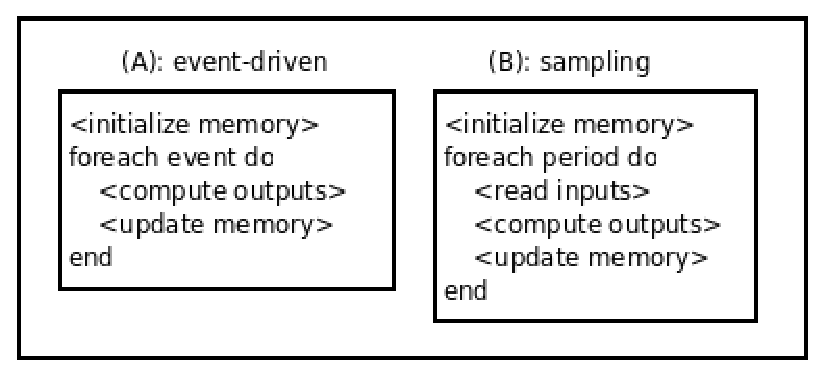
\includegraphics[width=3.0in]{sync_impl.eps}
\caption{Schedulers for synchronous systems}
\label{fig:concurrency.sync.impl}
\end{figure}

Figure \ref{fig.impl} shows two common implementation schemes for synchronous 
schedulers~\cite{rp.twelve}.
%
In the event-driven scheme, a loop iteration computes outputs for each event 
occurrence.
%
In the sampling scheme, a loop iteration computes the inputs and outputs for 
each clock tick.
%
In both cases, each loop iteration represents a logical instant in which the 
system as a whole reacts synchronously before going to next instant.
During a reaction, the environment is invariant, possibly buffering incoming 
input events to be processed further.
%
Both schemes are compliant with the synchronous hypothesis, in which input and 
resulting output happen at the same time (in this notion of time as a sequence 
of discrete events or clock ticks).

The asynchronous execution model is more general and does not make assumptions 
of implicit synchronization.
Each entity in the system (e.g., a thread or actor) is independent from one 
another and executes at its own speed.
In order to coordinate at specific points, they require explicit 
synchronization primitives (e.g., mutual exclusion or message passing).
% ADA, thread-based concurrency, CSP

For structured reactive programming, we argue that the synchronous model is 
more appropriate.
%
Below, we show how the synchronous model can handle two desired properties 
considering concurrent activities: \emph{deterministic execution} and 
\emph{orthogonal abortion}.

both yield to better reasoning
behave the same with or without

to show that
We focus on the composition of concurrent activities, given

In our work we use the synchronous model.
for concurrency
most difficult is composing activities

focus on synchronous vs asynchronous compositions

Figure~\ref{lst.leds} shows three implementations for an application that 
blinks two LEDs in parallel with different frequencies.
We implemented it in two asynchronous languages 
(actor-based~\cite{arduino.occam} and thread-based~\cite{arduino.chibios}, and 
also in a synchronous language with \CEU.
%
The intent and syntactic structure of the implementations is very similar:
composing in parallel the two blinking activities.
%
The LEDs should blink together every 3 seconds (\emph{least common denominator} 
between 600ms and 1s).
%
As we expected, the LEDs in the two asynchronous implementations loose 
synchronism after some time of execution, while \CEU implementation remains 
synchronized forever.
%
The example highlights how the inherent non-determinism in the asynchronous 
model makes hard to compose activities supposedly synchronized:
in the first example, unpredictable latency in message passing;
in the second example, unpredictable scheduling.
%
In \CEU, \code{await} is the only primitive that takes time and is XXX with the 
problem specification: the internal timings for communication and computation 
is neglected in accordance to the synchronous hypothesis.


Although this application can be implemented correctly with an asynchronous 
execution model, it circumvents the language style, as timers need to be 
synchronized in a single thread.

, each blinking a different LED in a loop (simulates a loop with .

but not the semantics

\begin{figure}[t]
\begin{minipage}[t]{0.34\linewidth}
\begin{lstlisting}
// OCCAM-PI
PROC main ()
 CHAN SIGNAL s1,s2:
 PAR
  PAR
   tick(600, s1!)
   toggle(11, s1?)
  PAR
   tick(1000, s2!)
   toggle(12, s2?)
:

\end{lstlisting}
\end{minipage}
%
\begin{minipage}[t]{0.33\linewidth}
\begin{lstlisting}
// ChibiOS
void thread1 () {
  while (1) {
    sleep(600);
    toggle(11);
  }
}
void thread2 () {
  while (1) {
    sleep(1000);
    toggle(12);
  }
}

void setup () {
  create(thread1);
  create(thread2);
}

\end{lstlisting}
\end{minipage}
%
\begin{minipage}[t]{0.31\linewidth}
\begin{lstlisting}
// Ceu
par do
  loop do
    await 600ms;
    _toggle(11);
  end
with
  loop do
    await 1s;
    _toggle(12);
  end
end
\end{lstlisting}
\end{minipage}
%
\rule{14cm}{0.37pt}
\caption{ Two blinking LEDs in OCCAM-PI, ChibiOS and \CEU.\newline
{\small %\textmd{
Each line of execution in parallel blinks a LED with a fixed (but different) 
frequency.
(The LEDs are connected to I/O ports 11 and 12.)
Every 3 seconds both LEDs should light on together.
After a couple of minutes of execution, only the implementation in \CEU remains 
synchronized.
}%}
\label{lst.releds}
}
\end{figure}

On the one hand, xxx
determinism
reasoning
%
On the other hand, the synchronous hypothesis does not hold for reactions that 
have latency (e.g., network communication or algorithm-intensive computations),

On the other hand, execution depends on the order
 reactions
because reaction to events do not interleave in complex

parallelism
latency

For reactive systems zzz
For highly synchronous systems, the sole synchronization overhead, which is 
non-existent in XXX, may neutralize any gains with parallelism.
% or even worsen parallelism

Illustrate with two examples:
that explore the advantages of synchronous:
reasoning in concurrency
seamless composition
    abortion takes *at most* one tick
    alternatives strong/weak, but *at most* one tick
    async may take time (unresponsive in the meantime!)
    even if you simulate with communication, it will take time

CSP has only syntactic support for the *and* semantics
p-threads discourages exit
Java threads deprecated Exit

                 .: determinism and

1-determinism/synchronism
2-composition

communitacions is directed and takes time (because the receiver may not be 
waiting)

The synchronous model
input => output
broadcast possible
global consensus possible
determinism
simpler model

In synchronous systems, communication is instantaneous.
The zero-delay property of the synchronous hypothesis guarantees that no time 
elapses between event announcement and receiving.
Also, as communication is via broadcast, all systems parts share the same 
information all the time.
These two characteristics make global data consensus another property of 
synchronous systems.


hypothesis fail on
however, does not apply when the computation involves latency:
problem communication takes time
either communication or time consuming operations
because now, at the speed of the program

Termination and abortion:
the real problem with the asynchronous model
implies
heap-based objects

Two examples:
termination / memory / no composition
time elapse / non-determinism / analogia do elevador

conclusion:
no blind/free/orthogonal composition
no deterministic/reproducible execution
parallelism / no-forced synch
time-consuming / independent


Both seminal works propose synchronous languages
statecharts and Esterel
so we call the
synchrnous reactive model

to contrast with interactive or the new asynchronous reactive model

A recent

important distinction from interactive is only the "environment speed"
a huge difference as it implies...

This definition is not the same as today:

The meaning of Reactive


synchronous reactive
vs
asynchronous reactive

berry classification
bash asynchronous
compositions
PAR/OR
not really parallel

diagrama com as duas formas de implementacao
mostrar que em ambas, apenas um evento eh tratado
"of course that reactions can trigger time-consuming operation that last 
multiple reactions, but it is important to recognize that the programmer is 
consious about that..."

Berry classified reactive applications as...
From this, he denied threads (ada, now threads) and also CSP-like languages 
where communication is point-wise and takes time (csp, now erlang)
asynchronous execution or asynchronous communication (with latency)

in terms of communication
- broadcast (single global vision of an event)
- p2p (loose simultaneity when simulating broadcast

\section{Structured Reactive Programming}
\label{sec.reactive}

- await, sequence, vars
- parallel, patterns, ortoghonal
- finalize for C integration and keep orthogonality
- organisms, static, dynamic. do T;

\section{Related work}

- asynchronous langs
- Esterel + descendants
- CRP
- simula
- FRP

interactive  vs reactive
asynchronous vs synchronous
dataflow vs control
dynamic vs static

imperative
    - sequential (eliminates state machines)
    - better resource control
    - less abstract

dataflow

exemplo data melhor vs control melhor

The synchronous concurrency model...

We show composibility, sequential, imperative
safety
Then, we extend synchronous reactive programming with dynamic

control vs data reactivity

\begin{comment}
===============================================================================

In computing, reactive programming is a programming paradigm oriented around data flows and the propagation of change. This means that it should be possible to express static or dynamic data flows with ease in the programming languages used, and that the underlying execution model will automatically propagate changes through the data flow.

For example, in an imperative programming setting, a := b + c would mean that a is being assigned the result of b + c in the instant the expression is evaluated. Later, the values of b and c can be changed with no effect on the value of a.

In reactive programming, the value of a would be automatically updated based on 
the new values.

===============================================================================

There seems to be a lot of confusion about Reactive Programming. What is it? Who created it?

The earliest reference I could find was written by Gérard Berry (one of the creators of the Esterel dataflow language) in his 1989 paper, “Real time programming: Special purpose or general purpose languages.” I emailed him to see if he knew of an earlier use. Mr. Berry pointed me to the 1985 paper, “On the development of reactive systems” by David Harel and Amir Pnueli. After contacting Professor Harel, he confirmed that they where the originators of the term.

So it would seem that Reactive Programming is at least 30 years old.

Harel and Pnueli’s paper discussed designing reactive systems in general, software or hardware. Their definition was…

    “Reactive systems… are repeatedly prompted by the outside world and their role is to continuously respond to external inputs.”

    D. Harel and A. Pnuli, “On the Development of Reactive Systems” (1985)

Mr. Berry’s paper focused on the software aspects of Reactive Programming…

    “It is convenient to distinguish roughly between three kinds of computer programs. Transformational programs compute results from a given set of inputs; typical examples are compilers or numerical computation programs. Interactive programs interact at their own speed with users or with other programs; from a user point of view a time-sharing system is interactive. Reactive programs also maintain a continuous interaction with their environment, but at a speed which is determined by the environment, not by the program itself. Interactive programs work at their own pace and mostly deal with communications, while reactive programs only work in response to external demands and mostly deal with accurate interrupt handling.

    Real-time programs are usually reactive. However, there are reactive program that are not usually considered as being real-time, such as protocols, system drivers or man-machine interface handlers. All reactive programs require a common programming style.

    Complex applications usually require establishing cooperation between the three kinds of programs. For example, a programmer uses a man-machine interface involving menus, scroll bars and other reactive devices. The reactive interface permits him to tell the interactive operating systems to start transformational computations such as program compilations.”

    Berry, Gérard. “Real time programming: Special purpose or general purpose languages.” (1989)

From the preceding quotes we can say that reactive programs…

    Activate in response to external demands
    Mostly deal with handling parallelism
    Operate at the rate of incoming data
    Often work in cooperation with transformational and interactive aspects

The definition of dataflow is a little more vague. Any system where the data moves between code units and triggers execution of the code could be called dataflow, that includes reactive systems. Thus, I consider Reactive Programming to be a subset of dataflow but a rather large subset. In casual use, Reactive Programming it is often a synonym for dataflow.

In more recent years Reactive Programming has become associated with two elements. Microsoft’s Reactive Extensions and Typesafe’s Reactive Manifesto.

Some people believe that Erik Meijer (formerly of Microsoft) and Jonas Bonér (of Typesafe) are trying to claim an old idea and call it their own. I am quite sure both of them are very aware of all of the previous work that has gone into Reactive Programming and dataflow. Mr. Bonér wrote about his observations on the resurgence of old techniques to solve new problems…

    “…Over the last few years we have seen quite a few different techniques and tools emerge in the industry as a way to address these new requirements. Some of them are old and proven, but to a large extent forgotten techniques, while others are novel and creative.”

    Why Do We Need a Reactive Manifesto

Reactive Programming and dataflow are old ideals that are being rediscovered because they help us solve problems we currently face.
\end{comment}

Adding dynamic state and references to SRP is a significant contribution.  
However the presentation assumes the audience already appreciates the 
advantages of SRP over standard imperative semantics. Most observers will not 
notice the difference at all and think this is just a weird syntactic sugar for 
standard multithreaded programming. SRP needs to be better explained and 
justified, perhaps by showing how it simplifies the examples.

\CEU is a Esterel-based reactive language that targets constrained embedded 
platforms.
%
Relying on a deterministic semantics, it provides safe shared-memory 
concurrency among lines of execution.
%
\CEU introduces a stack-based execution policy for internal events which 
enables advanced control mechanisms considering the context of embedded 
systems, such as exception handling and a limited form of coroutines.
%
The conjunction of shared-memory concurrency with internal events allows 
programs to express dependency among variables reliably, reconciling the 
control and dataflow reactive styles in a single language.
%As far as we know, \CEU is the first language to reconcile the control and 
%dataflow reactive styles.
%
%We present a formal description of \CEU and show how its synchronous and 
%static nature enables a compile-time analysis to ensure that reactions to the 
%environment are deterministic and execute with bounded memory and CPU time.
\end{abstract}

%\category{CR-number}{subcategory}{third-level}
\category{D.3.1}{Programming Languages}{Formal Definitions and Theory}
\category{D.3.3}{Programming Languages}{Language Constructs and Features}

\terms{Design, Languages}

\keywords{Concurrency, Dataflow, Determinism, Embedded Systems, Esterel, 
Synchronous, Reactivity}

\bibliographystyle{abbrv}
\bibliography{other,my}

\end{document}
